    \section*{Gaining intuition about feature transformations}

        Now that we understand the general idea of feature transformations, we can begin work with them, particularly for classification.

        Our goal is often to take data that linear models couldn't handle, and make it \textbf{separable.} 

        So, we'll consider maybe the simplest (solvable) case of a nonlinear data set:

        \begin{figure}[H]
            \centering
            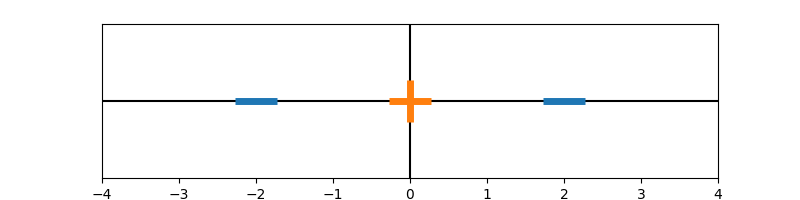
\includegraphics[width=120mm,scale=0.5]{images/feature_images/inseparable.png}
        \end{figure}

        In its current state, there's no one plane that would go through these data points: this is where our transform comes in. We'll try using a polynomial transform with $x^2$. It turns out, $-x^2+2$ works pretty well.

        How do we visualize this? It turns out, there are different perspectives:\\

        \begin{clarification}
            There are \gren{two} different ways we can \vocab{graph} a transformation:
            \begin{itemize}
                \item We transform the \purp{separator}: if our model is $-x^2+2$, we just graph that function over the data.
                    \begin{itemize}
                        \item This is the approach we used above: we wanted a line that \gren{fit} to our data.
                    \end{itemize}
                \item We transform the \purp{data}: we graph each data point according to our model $-x^2+2$.
                    \begin{itemize}
                        \item This model allows us to keep a "\gren{linear} separator": we effectively "shift" the data to be linear.
                    \end{itemize}
            \end{itemize}

            These models are mathematically \gren{equivalent}, and we'll switch the approach we're using based on which is easier/more useful to graph.
        \end{clarification}

        It may seem concerning to transform the data, rather than the model. However, keep in mind that:

        \begin{itemize}
            \item If you switch perspectives, they're the same: a different model will just "transform" the data when calculating its output.
            
            \item Usually, we try to preserve the original structure of the data, so we don't lose information: we just add more.
                \begin{itemize}
                    \item For example, $[1,x,x^2]$ still contains the information $x$: we just add $x^2$.
                \end{itemize}
        \end{itemize}

        \miniex Let's show both of these in action.

        \subsecdiv

        \subsection*{Transforming our separator}
    
            First, we transform our linear separator as desired: graphing $-x^2+2=0$ on our plot. 
    
            \begin{figure}[H]
                \centering
                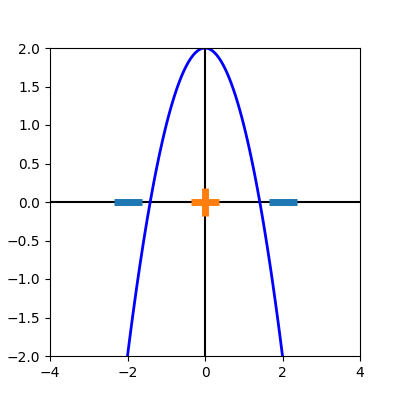
\includegraphics[width=60mm,scale=0.5]{images/feature_images/nonlinear_separator.png}
                \caption*{In this version, we've taken our hyperplane separator and transformed it nonlinearly.}
            \end{figure}
    
            In this case, we have assigned $-x^2+2<0$ as positive.
    
            In this version, we preserve the structure of the data, making it easier to see the original shape. However, it's not as easy to think about the shape and orientation of the "plane" now that it's been deformed. 
            
            For example, we don't really have a good "normal" vector, even if we know which side is positive. This is why, to keep our model "linear", we can transform the data, and find the corresponding plane. We'll do that next.
    
            \subsecdiv

        \subsection*{Transforming our data}
    
            In this case, every data point gets plotted on $[x,x^2]$. Our hyperplane is given by 
    
            \begin{equation}
                -x^2+2 = 
                \overbrace{
                \begin{bmatrix}
                    0 \\ -1
                \end{bmatrix}^T
                }^{\theta^T}
                \begin{bmatrix}
                    x \\ x^2
                \end{bmatrix}
                + 2
            \end{equation}
    
            Thus, we get a $\theta$ pointing downward, with an offset of 2.
    
            \begin{figure}[H]
                \centering
                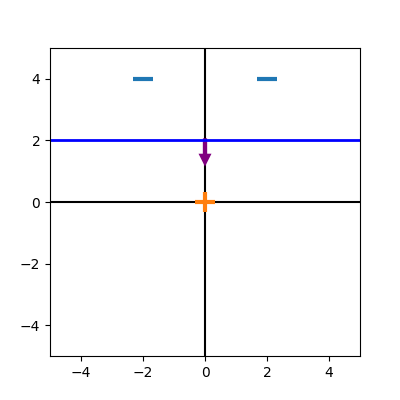
\includegraphics[width=60mm,scale=0.5]{images/feature_images/nonlinear_data.png}
                \caption*{This time, we've transformed our data: the math is totally the same, but now we can identify our separator more easily.}
            \end{figure}
    
            Note that our transformation makes the data linearly separable!\\
    
            \begin{concept}
                Features transformations allow us to \purp{non-linearly} transform our data, in order to make that data \vocab{linearly separable}, or at least, more \gren{accurate} with a linear separator.
    
                Often, we do this by transforming into a \purp{higher dimensional} space.
            \end{concept}
    
            \subsecdiv

        \subsection*{Positive vs. Negative}

            While these perspectives are helpful, they can become too complicated with more dimensions/higher-dimensional transformations.

            In an effort to simplify, we might ask ourselves, "what do we really want to know"? In the end, all we typically care about is classification: which data points are positive or negative?

            So, we'll create a third representation to correspond to that.\\

            \begin{concept}
                A third, \gren{simplified} representation of our transformation doesn't show how it affects our data points or classifier. Instead, we just show the \purp{result}: which regions are classified as positive, and which are classified as negative?

                This allows us to see which points get \gren{classified} in which way, without considering the high-dimensional details of the model itself.
            \end{concept}

            \miniex We can graph this for our sample data:

            \begin{figure}[H]
                \centering
                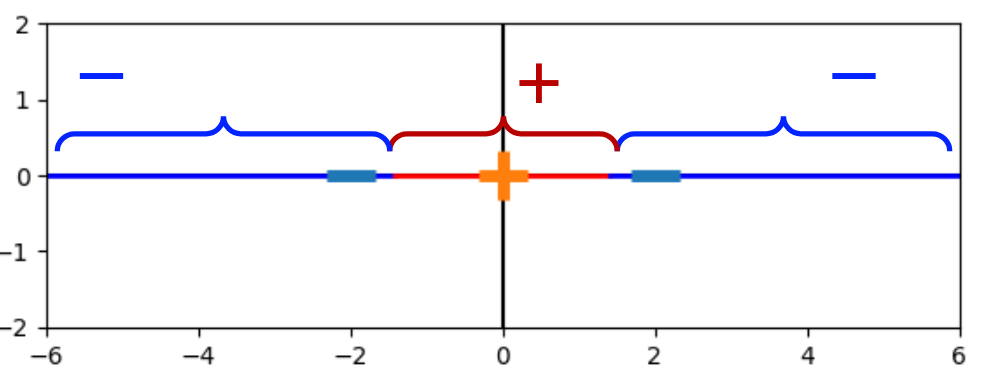
\includegraphics[width=100mm,scale=0.5]{images/feature_images/positive_negative_disp.png}
                \caption*{This way, we can stay in a 1-D space, while showing the information we need!}
            \end{figure}

            Note that the points where we switch between positive and negative, $\pm \sqrt{2}$, are the points corresponding to $-x^2+2=0$: they're the only part of the separator surface visible in our 1D plot.
                \note{They match our nonlinear hyperplane separator from section* 5.1.1}


        \secdiv
